% Created 2021-01-24 Sun 22:49
% Intended LaTeX compiler: pdflatex
\documentclass[11pt]{article}
\usepackage[utf8]{inputenc}
\usepackage[T1]{fontenc}
\usepackage{graphicx}
\usepackage{grffile}
\usepackage{longtable}
\usepackage{wrapfig}
\usepackage{rotating}
\usepackage[normalem]{ulem}
\usepackage{amsmath}
\usepackage{textcomp}
\usepackage{amssymb}
\usepackage{capt-of}
\usepackage{hyperref}
\usepackage{minted}
\hypersetup{colorlinks=true, linkcolor=black, filecolor=red, urlcolor=blue}
\usepackage[turkish]{babel}
\author{Eren Hatırnaz}
\date{1 Haziran 2020}
\title{Yazılım Gündemi - 2020/21\\\medskip
\large 25-31 Mayıs 2020}
\hypersetup{
 pdfauthor={Eren Hatırnaz},
 pdftitle={Yazılım Gündemi - 2020/21},
 pdfkeywords={},
 pdfsubject={},
 pdfcreator={Emacs 27.1 (Org mode 9.3)},
 pdflang={Turkish}}
\begin{document}

\maketitle
\tableofcontents \clearpage\shorthandoff{=}

\begin{center}
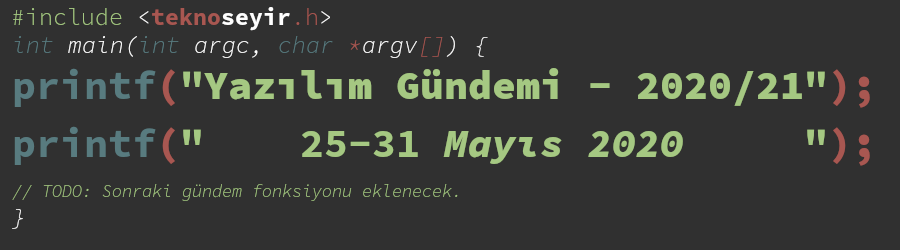
\includegraphics[width=.9\linewidth]{gorseller/yazilim-gundemi-banner.png}
\end{center}

\begin{center}
\href{../20/yazilim-gundemi-2020-20.pdf}{< Önceki Gündem} | \textbf{25-31 Mayıs 2020} | \href{../22/yazilim-gundemi-2020-22.pdf}{Sonraki Gündem >}

\href{https://teknoseyir.com/blog/yazilim-gundemi-2020-21}{TeknoSeyir'de Oku}
\end{center}

\section{\href{https://insights.stackoverflow.com/survey/2020}{StackOverflow Geliştirici Anketi 2020} sonuçları \href{https://stackoverflow.blog/2020/05/27/2020-stack-overflow-developer-survey-results/}{açıklandı}}
\label{sec:org3625313}
StackOverflow sitesinin her yıl düzenli olarak yaptığı geliştirici anketi bu
yılın Şubat ayında duyurulmuştu. Geçtiğimiz hafta içerisinde ise bu anketin
sonuçları yayınlandı. Yaklaşık 65.000 kişinin katıldığı bu ankete Türkiye'den
katılım oranı \textbf{\%1.22} çıkmış. Sektördeki en yaygın 3 rol ise tahmin
edebileceğiniz üzere şunlar: \textbf{Back-End Developer (\%55.2)}, \textbf{Full-Stack
Developer (\%54.9)} ve \emph{\textbf{Front-End Developer (\%37.1)}}. Ankete katılanların
çoğunluğu ise \textbf{\%26.5 ile 25-29 yaş arası insanlar} oluşturuyormuş.
Teknolojilerle ilgili diğer sonuçlar ise şu şekilde:

\subsection{En popüler programlama, betik ve işaretleme dilleri sıralaması}
\label{sec:orgb9b066d}
\begin{center}
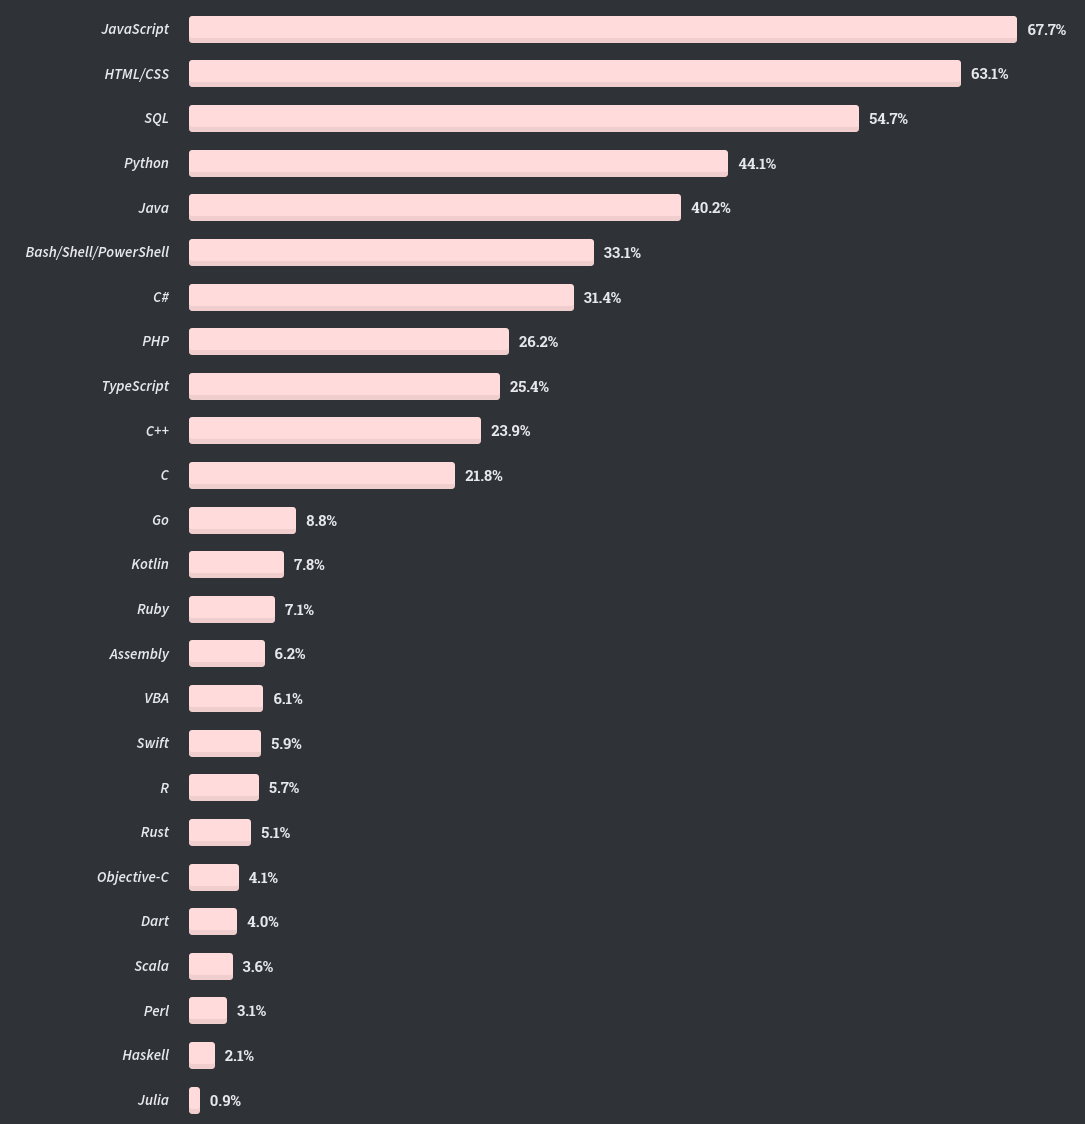
\includegraphics[width=.9\linewidth]{gorseller/stackoverflow-2020-populer-diller.png}
\end{center}
\subsection{En popüler web framework'leri}
\label{sec:org021837b}
\begin{center}
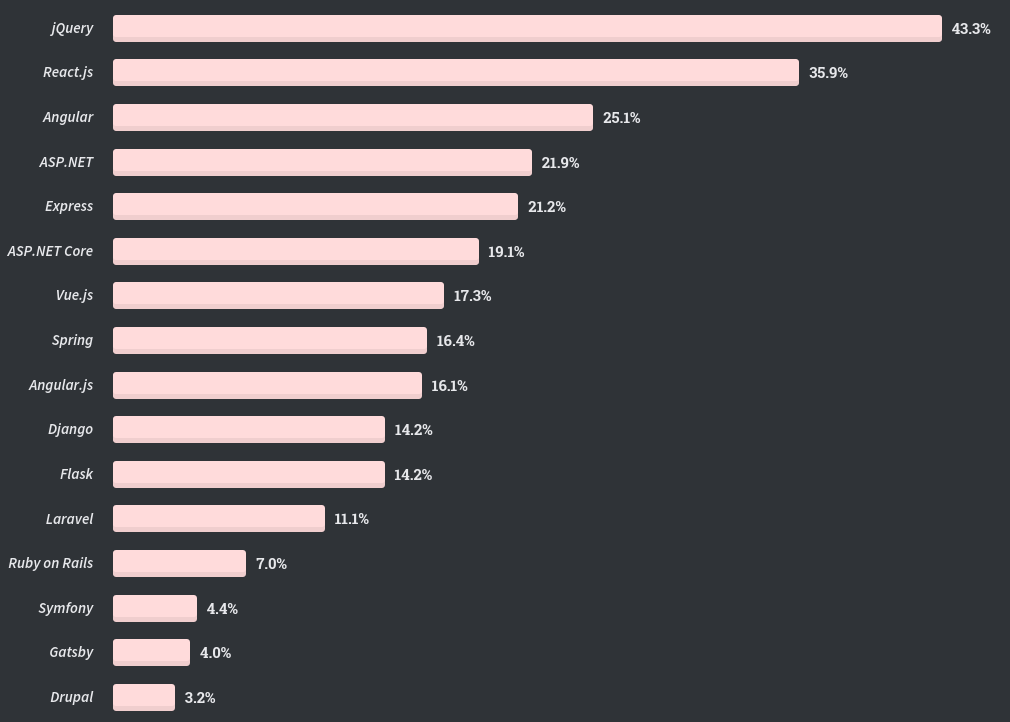
\includegraphics[width=.9\linewidth]{gorseller/stackoverflow-2020-web-frameworks.png}
\end{center}
\subsection{En çok sevilen ve nefret edilen programlama dilleri}
\label{sec:org1cb4d52}
\begin{figure}[htbp]
\centering
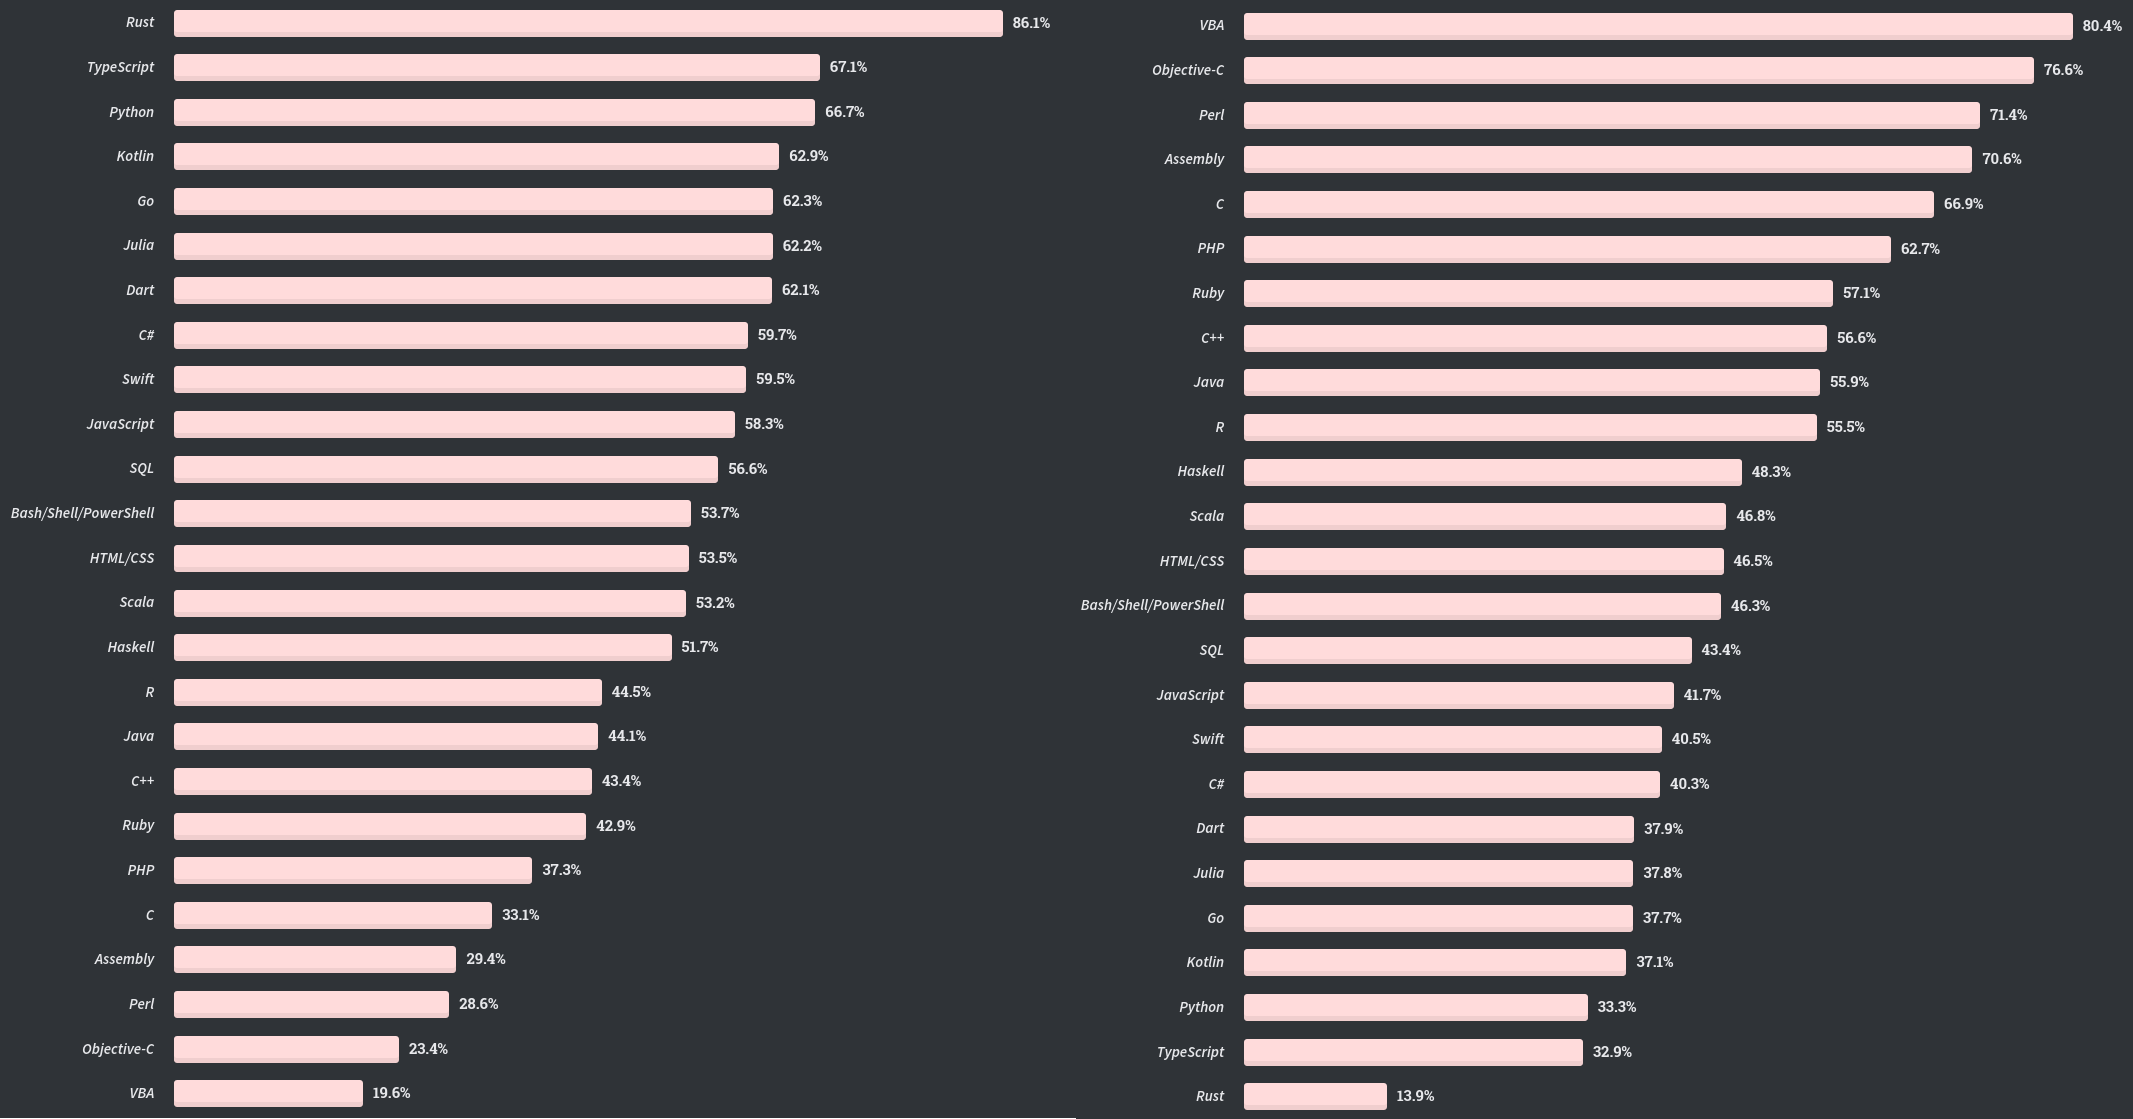
\includegraphics[width=.9\linewidth]{gorseller/stackoverflow-sev-nefret.png}
\caption[\textbf{(SAĞ):}]{\textbf{(SOL):} En çok sevilen programlama dilleri. \\
 \textbf{(SAĞ):} En çok nefret edilen programlama dilleri}
\end{figure}

Bu tarz konuları değerlendirirken sürekli söylediğim bir şeyi yine tekrarlamak
isterim: Teknoloji tercihlerinizi bu anketlerin sonuçlarına göre değil kendi
ihtiyaçlarınıza göre yapın. Bu veriler sadece geliştirici ekosisteminin büyük
resmini görmeye yarıyor.

Anketin tüm sonuçlarını buraya eklemek mümkün olmadığı için sadece bu
başlıkları aldım ben ama diğer sonuçlar da oldukça ilgi çekici. StackOverflow
da zaten sonuçlar için çok güzel bir sayfa hazırlamış. Konu başlığına
eklediğim bağlantıya tıklayarak diğer anket sonuçlarını inceleyebilirsiniz.
\section{Microsoft'un paket yöneticisi WinGet, \href{https://www.theverge.com/2020/5/28/21272964/microsoft-winget-windows-package-manager-appget-copied}{AppGet'den 'esinlenmiş'}}
\label{sec:org363efbe}
Bir önceki yazılım gündemi yazısında (bkz: \href{../20/yazilim-gundemi-2020-20.pdf}{Yazılım Gündemi - 2020/20}) sizlere
Microsoft'un Build 2020 etkinliğinde duyurduğu paket yöneticisi WinGet'den
bahsetmiştim. Yine aynı hafta içerisinde AppGet isimli farklı bir paket
yöneticisinin de geliştiricisi tarafından artık \href{https://keivan.io/the-day-appget-died/}{devam ettirilmeyeceği
duyurulmuştu} fakat bunu gündeme eklememiştim (İtiraf etmek gerekirse
geliştiricinin yayınladığı yazıyı okumadığım için konuyu farklı bir şey
sanmıştım). Bu hafta The Verge sitesinde yayınlanan haber ve Microsoft'un
ilgili takımının yöneticisinin \href{https://devblogs.microsoft.com/commandline/winget-install-learning/}{yayınladığı yazıyla} birlikte konu daha fazla
gündeme geldi.

AppGet'in geliştiricisi Keivan Beigi, geçtiğimiz hafta bir blog yazısıyla
AppGet'i artık geliştirmeyeceğini, 1 Ağustostan itibaren de kapatacağını
duyurdu. Bu hareketinin nedenini ise şöyle açıkladı: "Microsoft WinGet'i
geliştirirken benimle iş görüşmesi yaptı, ben onlara AppGet'in arka planından
ve teknik kısımlarından bahsedip, gelecekle ilgili fikirlerimi aktardım fakat
sonrasında bana hiç geri dönüş yapmadılar. Geçtiğimiz hafta duyurulan WinGet'i
görünce çok oldum. Microsoft'la rekabet edemem ve topluluğu da bölmek
istemiyorum. O yüzden AppGet'i artık geliştirmeyeceğim". Üstelik WinGet'in
duyuru yazısının hiçbir yerinde de bu geliştiriciden ve emeğinden
bahsedilmemiş.

Olayın Reddit ve HackerNews gibi platformlarda gündem olmasının ardından olaya
konu olan Microsoft takımının yöneticisi açıklama yapmak zorunda kaldı ve
yaptıklarını bir nevi kabul edip, AppGet'deki şu şeylerden esinlendik gibi bir
yazı yazıp Keivan Beigi'ye teşekkür etmiş. "Geç gelen adalet, adalet değildir"
atasözünü şu şekilde değiştirirsek konuya çok uyumlu oluyor: "Geç gelen
teşekkür, teşekkür değildir".

Geçmişteki Microsoft davranışlarının terk edilip, açık kaynağa yaklaşmalarının
ardından böyle bir haberle gündeme gelmeleri hiç iyi olmadı. Açıkcası ben de
Microsoft'un artık bakış açısını değiştirdiğini düşünüyordum fakat bu olay ve
sonrasında yaşananlar bende hiç iyi bir intiba bırakmadı.
\section{SpaceX Dragon 2 kapsülünün uçuş arayüzü Chromium üzerinde \href{https://space.stackexchange.com/questions/9243/what-computer-and-software-is-used-by-the-falcon-9/9446\#9446}{JavaScript çalıştırıyormuş}}
\label{sec:org5aea381}
Geçtiğimiz hafta içerisinde 2011'den beri ilk defa Amerikan topraklarından
astronot gönderildi. Bu görevin diğerlerinden farklı ve özel bir yanı daha
var: Tarihte ilk kez özel bir şirket uzaya insan gönderdi. Çoğumuz zaten NASA
ve SpaceX tarafından yapılan canlı yayını izlemiştir. İşte bu yayınlarda
gördüğümüz SpaceX Dragon 2 kapsülünün dokunmatik uçuş arayüzü Chromium
üzerinde çalışan bir arayüzüymüş. Bunu da 2015'yılında StackExchange sitesinde
sorulmuş bir soruya verilmiş cevaptan öğreniyoruz. Cevabı yazan kişinin
kaynağı ise Google Developer Conferance 2015 ve 2016'de SpaceX mühendisleri
ile olan konuşmasıymış.

\begin{figure}[htbp]
\centering
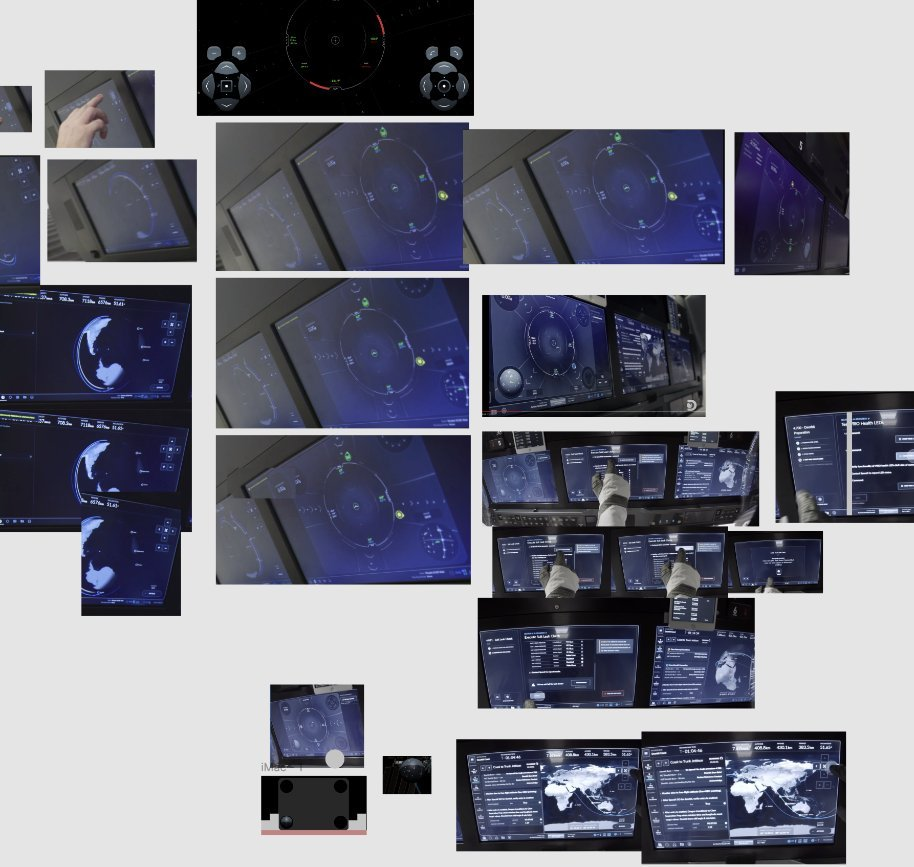
\includegraphics[width=.9\linewidth]{gorseller/spacex-dragon-ucus-arayuzu.jpeg}
\caption{SpaceX canlı yayınından alınmış, çeşitli açılardan Dragon 2 kapsülünün uçuş arayüzü görselleri}
\end{figure}

Bir kişinin bulup Reddit ve HackerNews gibi platformlarda paylaşması üzere
konu üzerine bayağı bir espri yapıldı. SpaceX mühendisleri mutlaka
JavaScript'in yol açabileceği şeylerin önüne geçecek önemleri almıştır tabii
ki, zaten uzun yıllardır test edilen kapsül geçtiğimiz hafta sorunsuz bir
şekile Uluslararası Uzak İstasyonuna kenetlendi ve astronotları sağlıklı
şekilde taşıdı. Dragon 2 kapsülünün kenetlenme ekranının bir benzeri için şu
adresdeki simülasyonu deneyebilirsiniz: \url{https://iss-sim.spacex.com/} (arkaya da
Interstellar filminin meşhur müziğini açarsanız daha eğlenceli oluyor :))

İlgili StackOverflow cevabından öğrendiğimiz diğer bilgiler ise Falcon 9
roketi hakkında. Falcon 9 roketinin C/C++ dilleri kullanılarak oluşturulmuş
yazılımı kendilerine göre özelleştirdikleri Linux çekirdeği üzerinde 3 farklı
işlemcide çalışıyormuş ve sonuçlar karşılaştırılıp uyumsuzluk durumlarında
işleme alınmıyormuş.

Ayrıca benim de bu hafta keşfettiğim SpaceX API'sini de sizlerle paylaşmak
isterim. Bu hafta içerisinde Dragon kapsülleri için de birçok end-point
kullanıma sunulmuş: \url{https://docs.spacexdata.com/}.
\section{Android Studio \href{https://android-developers.googleblog.com/2020/05/android-studio-4.html}{4.0 sürümü yayınlandı}}
\label{sec:org8a8a75c}
IntelliJ IDEA temelli, Google tarafından geliştirilen Android Studio IDE'sinin
geçtiğimiz hafta içerisinde 4.0 numaralı sürümü stable etiketiyle birlikte
yayınlandı. Bu sürümle birlikte gelen birkaç özelliği birlikte inceleyelim:

\subsection{Motion Editor}
\label{sec:org42453e6}
\url{gorseller/android-studio-4-0-motion-editor.gif}

Android işletim sisteminin 4.0 sürümünden beri desteklenen \texttt{MonitonLayout}
API'si sayesinde objelere animasyon kazandırabiliyorduk zaten ama artık
Android Studio 4.0 ile bu daha kolay bir hale geldi. Özel editör sayesinde
artık XML dosyalarıyla boğuşmadan grafik arayüzünü kullanarak animasyonlar
yaratabileceğiz. İsterseniz yine XML görünümüze geçebiliyorsunuz tabii.
\subsection{Layout Validation}
\label{sec:orgcc9f237}
Android sistemler için uygulama geliştirirken tek bir cihaz olmamasından
dolayı birçok farklı ekran boyutu için tasarımınızı ayarlamanız gerekiyor
(web tarafındaki responsive tasarım gibi). Artık Android Studio 4.0 ile
birlikte her cihaz için farklı emülatör çalıştırmak yerine \textbf{Layout
Validation} sekmesini kullanarak tasarımınızın farklı ekran boyutlarında
nasıl gözüleceğini görebiliyorsunuz.

\begin{center}
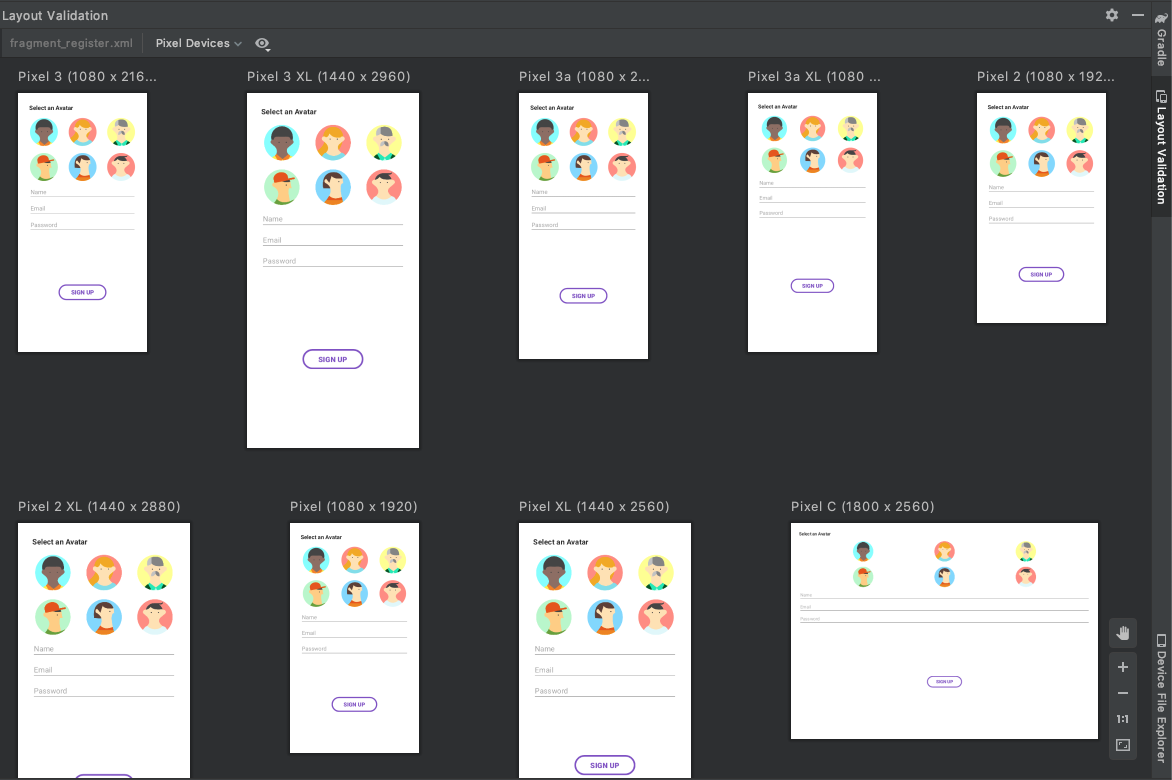
\includegraphics[width=.9\linewidth]{gorseller/android-studio-4-0-layout-validation.png}
\end{center}
\subsection{Build Analyzer}
\label{sec:org883250e}
Geliştirdiğiniz uygulamaları derlerken bazen derleme süreleri acayip
uzayabiliyor fakat bunun hangi eklenti ya da kütüphaneden kaynaklandığını
bulmak biraz zordu. Bu sürümle birlikte gelen \textbf{Build Analyzer} ile artık uzun
süren build işlemlerinde sorunlu olan eklenti ya da kütüphaneleri kolaylıkla
tespit edebileceksiniz.

\begin{center}
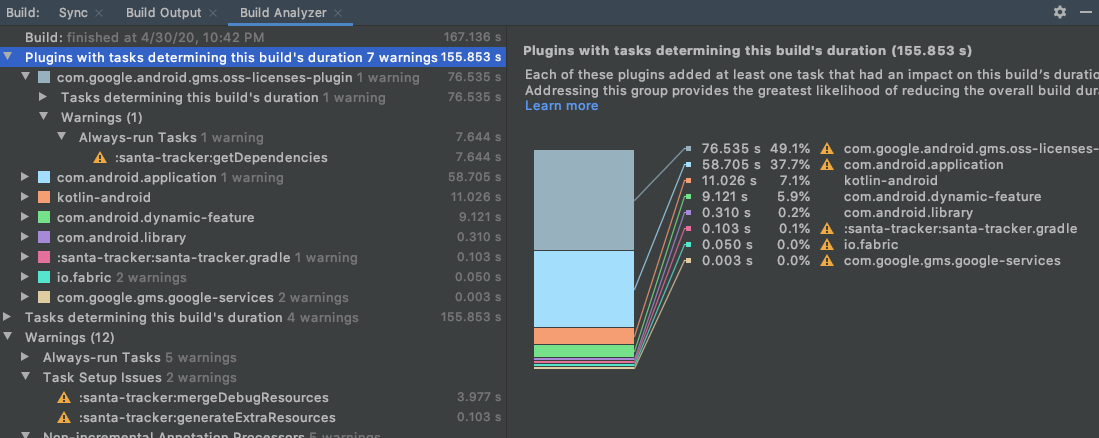
\includegraphics[width=.9\linewidth]{gorseller/android-studio-4-0-build-analyzer.png}
\end{center}

Android Studio'nun bu sürümüyle birlikte gelen diğer özellikler ve
değişiklikler için konu başlığına eklediğim bağlantıya tıklayabilir ya da
Android Developers kanalında yayınlanan \href{https://www.youtube.com/watch?v=f1fHPqAYj5I}{şu videoyu izleyebilirsiniz}.
\section{Google Chrome takımının nedensiz eklenti kaldırmalarının \href{https://kodfabrik.com/journal/why-am-i-shutting-down-kozmos}{yeni kurbanı: Kozmos}}
\label{sec:org416ebd4}
2016 yılındaki \texttt{left-pad} olayıyla tanıdığımız Azer Koçulu, npm'den sonra bu
sefer de Google Chrome Eklenti Takımı'ndan haksızlık gördü. \texttt{left-pad} olayını
hatırlamayanlar için Azer Koçulu'nun kendi sitesinde yazdığı \href{https://kodfabrik.com/journal/i-ve-just-liberated-my-modules}{şu yazıya} göz
atabilirler (\href{https://medium.com/@eserozvataf/azer-ko\%25C3\%25A7ulu-kik-left-pad-ve-npm-ed7c3098ecfb}{alternatif Türkçe kaynak}) ya da kendisinin konuk olduğu \href{https://www.youtube.com/watch?v=KjHLfDBVLFE}{şu
podcast yayını}na göz atabilirler. Bugünkü konumuz 2017'den beri geliştirmekte
olduğu ücretli Chrome eklentisi olan \href{https://getkozmos.com/}{Kozmos}.

\begin{center}
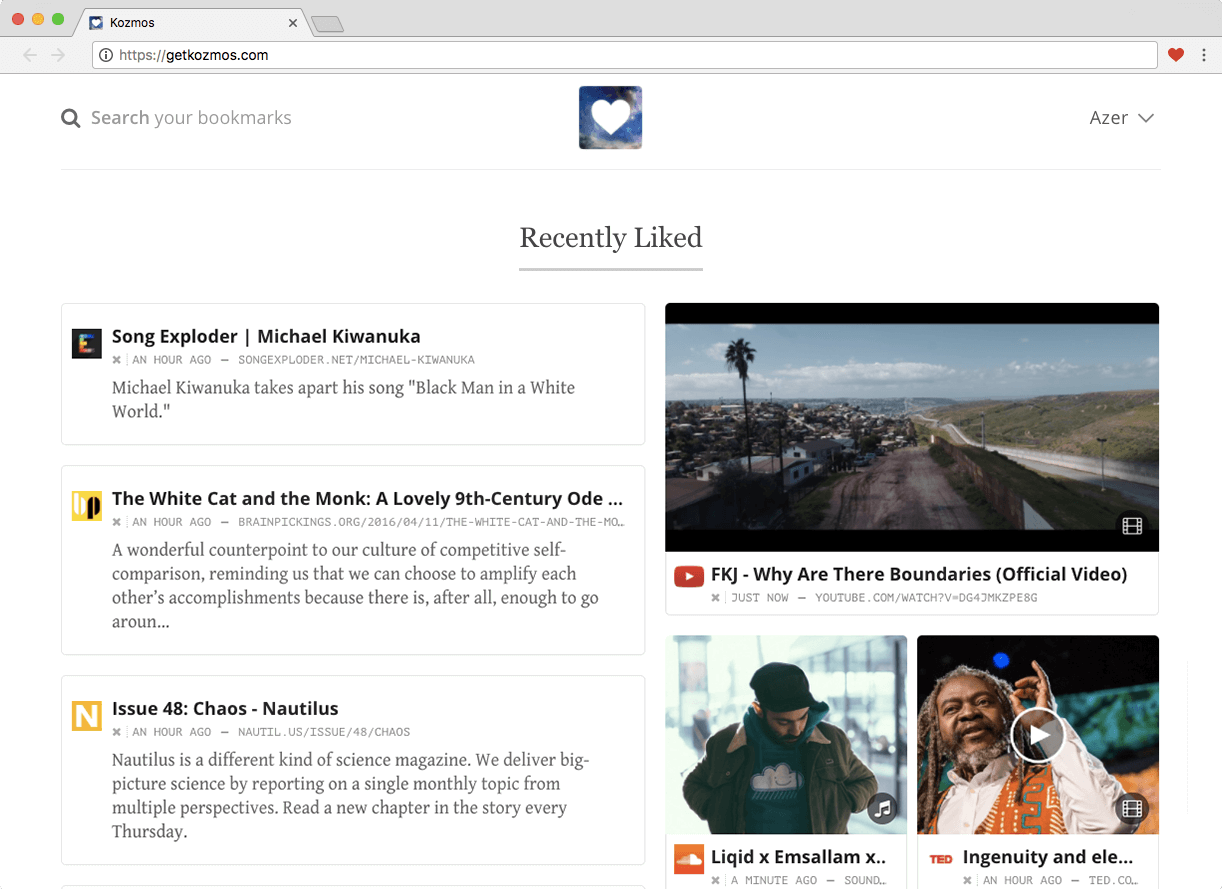
\includegraphics[width=.9\linewidth]{gorseller/kozmos.png}
\end{center}

Kısaca Kozmos, tamamen çevrimdışı çalışma imkanı sunan bir çeşit yerimi
depolama çözümüydü. İnternet bağlantınız yokken bilgilerinizi tarayıcının
içinde depolayan, internete bağlandığınızda ise her yerden erişebilmeniz için
onları kendi sunucularına gönderen bir yeni sekme sayfası eklentisiydi. Azer
Koçulu böyle bir girişimde bulunmuş fakat pek beklediği yatırımlara ulaşamamış
olsa da projeyi pasif gelir olarak sürdürmeye devam etmiş. Hiçbir kullanıcı
verisini satmamış, tamamen Google'ın Eklenti Marketi Kurallarına uygun
şekilde geliştirmesini yapmış.

Son 2 yıldır ise tabiri caizse Google'ın Chrome eklenti takımı Azer'in başına
musallat olmuş. Birkaç haftada bir eklentisini marketten kaldıran otomatik
botlar ile arasında şöyle bir diyalog geçirdikten sonra insan çalışanlar
durumu düzeltiyormuş (basit özet şeklinde):

\begin{quote}
\begin{itemize}
\item Google (Bot): Eklentini marketten kaldıracağız.
\item Azer Koçulu: Bu bir yanlışlık olmalı.
\item Google (Bot): Yanlışlıklık yok, kuralları gözden geçir, senin eklentin
kurallardan birini ihlal ediyor.
\item Azer Koçulu: Hiçbirini ihlal etmiyor, bu bir yanlışlık!
\item Google (sonunda insan): Özür dileriz, yanlışlık oldu.
\end{itemize}
\end{quote}

ve bu tarz konuşmalar sürekli tekrarlandığı halde doğru düzgün bir çözüm
sunulmamış. En sonunda da birkaç ay önce Google'ın Chrome eklenti takımı
Kozmos'u hiçbir uyarı ya da bilgi vermeden Kozmos'u marketten kaldırmışlar.
Üstelik iletişim kurup durum hakkında bilgi alınabilecek bir destek sistemi
bile yokmuş.

Üzerine planlar yaptığınız, az da olsa gelir elde ettiğiniz bir projeniz işte
böyle rahat bir şekilde Google tarafından fişi çekilebiliyor. Bu yazı geçen
hafta yayınlanmış olmasına rağmen bu haftanın gündemine almamın sebeplerinden
biri de Google'ın bu yüzünü sizlere tekrar göstermek istemem. Üstelik bu
olaylar Google'ın elinde tuttuğu tüm uygulama marketlerinde (özellikle Android
Play Store üzerinde)sürekli tekrarlanıyor. Google'a güvenerek yola çıkacak
olanlar bir kez daha düşünsün.

Bu konu hakkında siz ne düşünüyorsunuz? Yorumlar bölümünde konuşalım.
\section{Qt \href{https://www.qt.io/blog/qt-5.15-released}{5.15 LTS sürümü yayınlandı}}
\label{sec:org9e3735f}
C++ ile platformlar arası (cross-platform) uygulama geliştirmeye yarayan
kütüphane Qt, geçtiğimiz hafta içerisinde 5.15 sürümünü Uzun-dönem desteği
(Long-term Support) etiketiyle yayınladı. Bu yılın başında duyurdukları (bkz:
\href{../05/yazilim-gundemi-2020-05.pdf}{Yazılım Gündemi - 2020/05}) gibi LTS etiketli sürümler artık sadece kurumsal
lisansı olan müşterilerine sunuluyor. Önümüzdeki 3 yıllık periyotda destek
almaya devam edecek olan 5.15 sürümüyle birlikte gelen bazı yenilikler ise şu
şekilde:

\begin{itemize}
\item \textbf{3 boyutlu grafik API'lerinin soyutlanması}: Farklı işletim sistemlerinde
çalışan farklı grafik kütüphanelerinin yaygınlaşmasıyla birlikte Qt de,
cross-platform sözünü tutabilmek için artık sadece \href{https://www.khronos.org/opengl/}{OpenGL} kullanmayacak.
Onun yerine bu katmanı soyutlayarak (abstracting), \href{https://developer.apple.com/metal/}{Metal}, \href{https://www.khronos.org/vulkan/}{Vulkan} ve \href{https://docs.microsoft.com/en-us/windows/win32/direct3d12/direct3d-12-graphics}{Direct
3D 12} gibi farklı grafik kütüphaneleriyle de çalışılabilmesini mümkün kılan
Qt Rendering Hardware Interface (RHI) sistemini getiriyor.
\item \textbf{Qt Quick 3D}: Qt tabanlı uygulamalarda 3 boyutlu içerikleri kullanmayı
kolaylaştıracak bir araç için tam destek geldi. Benchmark Demosu için \href{https://www.youtube.com/watch?v=wuRH-lr\_XBA}{şu
YouTube videosunu izleyebilirsiniz}.
\item \textbf{\href{https://www.qt.io/blog/qt-design-studio-1.5-released}{Qt Design Studio 1.5}}: Bu araca da 3 boyutlu çalışmalar için özellikler
eklenmiş.
\item \textbf{\href{https://www.qt.io/blog/new-qml-language-features-in-qt-5.15}{Yeni QML özellikleri}}
\item \textbf{\href{https://doc.qt.io/qt-5/qtlottieanimation-index.html}{Qt Lottie} için tam destek}.
\item \textbf{Qt WebEngine artık Chromium 80 kullanıyor}.
\item Qt Network artk TLS 1.3 destekliyor.
\end{itemize}

Bu sürümle birlikte gelen diğer özellikler ve değişiklikler için konu
başlığına eklediğim bağlantıya tıklayabilir ya da 4 Haziran günü
gerçekleştirilecek olan şu webiner etkinliğine kayıt olabilirsiniz: \href{https://www.qt.io/events/qt-515-lts-built-to-last-1589807096}{Qt 5.15
LTS: Built to Last}.

Qt ile ilgili diğer haberler:
\begin{itemize}
\item Qt Online Installer \href{https://www.qt.io/blog/qt-online-installer-3.2.3-released}{3.2.3 yayınlandı}.
\item Qt 5.15 ile birlikte gelen \href{https://www.qt.io/blog/whats-new-with-qt-for-android}{Android için Qt yenilikleri}.
\end{itemize}
\section{Yaklaşan Online Etkinlikler}
\label{sec:orgbcb5b28}
\begin{longtable}{|p{9.5cm}|l|}
\hline
Etkinlik İsmi & Tarihi\\
\hline
\endfirsthead
\multicolumn{2}{l}{Önceki sayfadan devam ediyor} \\
\hline

Etkinlik İsmi & Tarihi \\

\hline
\endhead
\hline\multicolumn{2}{r}{Devamı sonraki sayfada} \\
\endfoot
\endlastfoot
\hline
\href{https://kommunity.com/devnot-yazilimci-bulusmalari/events/pythonu-yeniden-kesfetmek-django-framework-ile-restful-api-gelistirme-0456cd39}{Python'u Yeniden Keşfetmek: Django Framework ile RESTful API Geliştirme} & 1 Haziran 20:00\\
\href{https://kommunity.com/tracikkaynak/events/acik-seminer-26-gun-microservice-monoliths-vs-microservices-12-factor-apps-b27a33e1}{Açık Seminer 26. Gün: Microservice Monoliths vs Microservices 12 Factor Apps} & 2 Haziran 14:00\\
\href{https://kommunity.com/tracikkaynak/events/acik-seminer-27-gun-differences-between-openshift-kubernetes-3a8d8109}{Açık Seminer 27. Gün: Differences Between OpenShift \& Kubernetes} & 3 Haziran 14:00\\
\href{https://kommunity.com/tracikkaynak/events/acik-seminer-28-gun-0401f590}{Açık Seminer 28. Gün: DevOps Modernizasyonu} & 4 Haziran 14:00\\
\href{https://kommunity.com/tracikkaynak/events/acik-seminer-29-gun-devops-ve-sanallastirma-teknolojileri-ornekleri-94d0ef9f}{Açık Seminer 29. Gün: DevOps ve Sanallaştırma Teknolojileri Örnekleri} & 5 Haziran 14:00\\
\href{https://kommunity.com/tracikkaynak/events/acik-seminer-30-gun-80c296da}{Açık Seminer 30. Gün: Veri Analizi Süreçlerinde TRT'deki DevOps Kültürü} & 6 Haziran 14:00\\
\href{https://kommunity.com/cloud-and-serverless-turkey/events/kubernetes-hands-on-5-rbac-and-secret-management-280ed399}{Kubernetes Hands-On no.5: RBAC and Secret Management} & 7 Haziran 13:30\\
\hline
\end{longtable}
\section{Diğer Haberler}
\label{sec:org6037838}
\begin{itemize}
\item Hindistan kendi koronavirüs takip uygulamasını \href{https://techcrunch.com/2020/05/26/aarogya-setu-india-source-code-release/}{açık kaynak yaptı}. \href{https://github.com/nic-delhi/AarogyaSetu\_Android}{GitHub
Deposu}
\begin{itemize}
\item Hindistan koronavirüs uygulamasında hata bulana \href{https://www.theregister.com/2020/05/27/aarogya\_set\_open\_source\_bug\_bounty/}{ödül vereceğini açıkladı}.
\item Açık kaynak yapılan uygulamanın marketteki uygulama ile aynı \href{https://twitter.com/jackerhack/status/1266971326918455298}{olmadığına
dair iddialar mevcut}.
\end{itemize}
\item Fransa StopCovid uygulamasının bütün platformlardaki uygulamalarını \href{https://gitlab.inria.fr/stopcovid19}{açık
kaynak yaptı}.
\item Google, Amerika'daki protestolar nedeniyle Android \href{https://www.reuters.com/article/us-minneapolis-police-google-android/google-postpones-android-11-unveiling-amid-u-s-protests-idUSKBN2360AS}{11 Beta sürümünü
yayınlamayı erteledi}. \href{https://twitter.com/AndroidDev/status/1266589514937466880}{Duyuru Tweet'i}
\item Docker ve Microsoft iş birliklerini \href{https://techcrunch.com/2020/05/27/docker-expands-relationship-with-microsoft-to-ease-developer-experience-across-platforms/}{genişleteceklerini duyurdular}.
\item Özgür Yazılım Vakfı (FSF) tüm \href{https://jitsi.org/jitsi-meet/}{Jitsi Meet} ile tüm üyelerine ücretsiz \href{https://www.fsf.org/blogs/community/fsf-gives-freedom-respecting-videoconferencing-to-all-associate-members}{video
konferans hizmeti sağlamaya başlamadı}.
\item TechEmpower firması, \href{https://www.techempower.com/benchmarks/\#section=data-r19}{Framework Benchmarks Round 19} \href{https://www.techempower.com/blog/2020/05/28/framework-benchmarks-round-19/}{sonuçlarını yayınladı}.
\item Node.js \href{https://nodejs.org/en/blog/release/v12.17.0/}{v12.17.0 LTS sürümü yayınlandı}.
\item Symfony birçok dalda yeni sürüm yayınladı:
\begin{itemize}
\item \href{https://symfony.com/blog/symfony-5-1-0-released}{Symfony 5.1.0}
\item \href{https://symfony.com/blog/symfony-5-0-9-released}{Symfony 5.0.9}
\item \href{https://symfony.com/blog/symfony-4-4-9-released}{Symfony 4.4.9}
\item \href{https://symfony.com/blog/symfony-3-4-41-released}{Symfony 3.4.41}
\end{itemize}
\item OpenSSH \href{https://www.openssh.com/releasenotes.html}{8.3 sürümü yayınlandı}. Artık \href{https://arstechnica.com/information-technology/2020/05/dangerous-sha-1-crypto-function-is-about-to-die-in-ssh/}{SHA-1 desteklenmiyor}.
\item Swift takımı sunucu ekosistemi için \href{https://swift.org/blog/aws-lambda-runtime/}{yeni açık kaynak projesini tanıttı}:
\href{https://github.com/swift-server/swift-aws-lambda-runtime/}{Swift AWS Lambda Runtime}.
\item Visual Studio Code artık \href{https://github.com/microsoft/vscode/issues/33620\#issuecomment-635367046}{ARM64 platformunu destekliyor}.
\item Visual Studio Code için \href{https://blog.zeplin.io/introducing-zeplin-for-visual-studio-code-edbc922a5784}{Zeplin eklentisi tanıtıldı}.
\item Sublime Merge \href{https://www.sublimetext.com/blog/articles/sublime-merge-2-announcement}{2 sürümü yayınlandı}.
\item Yeni bir fonksiyonel programlama dili Alpha sürümüyle \href{https://functional.blog/2020/05/25/designing-a-functional-programming-language-yatta/}{duyuruldu}: \href{https://yatta-lang.org/}{Yatta}.
\href{https://github.com/yatta-lang/yatta}{GitHub Deposu}
\item Yeni bir platformlar arası (cross-platform) açık kaynak C++ framework'ü
\href{https://preshing.com/20200526/a-new-cross-platform-open-source-cpp-framework/}{duyuruldu}: \href{https://plywood.arc80.com/}{Plywood}. \href{https://github.com/arc80/plywood}{GitHub Deposu}
\item Upbound Cloud Community Preview \href{https://blog.upbound.io/announcing-upbound-cloud-community-preview/}{tanıtıldı}.
\item Snowpack \href{https://www.snowpack.dev/posts/2020-05-26-snowpack-2-0-release/}{2.0 sürümü yayınlandı}.
\item immudb \href{https://github.com/codenotary/immudb/releases/tag/v0.6.0}{v0.6.0 sürümü yayınlandı}.
\item go-micro \href{https://github.com/micro/go-micro/releases/tag/v2.8.0}{v2.8.0 sürümü yayınlandı}.
\item TiDB \href{https://github.com/pingcap/tidb/releases/tag/v4.0.0}{v4.0.0 sürümü yayınlandı}.
\item Astree \href{http://edeforas.free.fr/?p=305}{v1.22 sürümü yayınlandı}.
\end{itemize}
\section{Lisans}
\label{sec:org99233d0}
\begin{center}
\begin{center}

\includegraphics[height=1.5cm]{../../../img/CC_BY-NC-SA_4.0.png}
\end{center}

\href{yazilim-gundemi-2020-21.pdf}{Yazılım Gündemi - 2020/21} yazısı \href{https://erenhatirnaz.github.io}{Eren Hatırnaz} tarafından \href{http://creativecommons.org/licenses/by-nc-sa/4.0/}{Creative Commons
Atıf-GayriTicari-AynıLisanslaPaylaş 4.0 Uluslararası Lisansı} (CC BY-NC-SA 4.0)
ile lisanslanmıştır.
\end{center}
\end{document}
